\begin{fullwidth}
\chapter[TYPOGRAPHY]{Typography}
\label{chap:task}
\end{fullwidth}

\marginnote{\adforn{42} \Chapref{chap:introduction} \hfill \Chapref{chap:sota1} \adforn{43}}

\paragraph{Synopsis}
This chapter presents some typographical specificities of the model §\ref{sec:task:typo}. Last, it presents some type of lists §\ref{sec:pstask:list}.

% =======================================================

\section{Some hints on typography}
\label{sec:task:typo}

\subsection{Numbers}

For numbers, you can use oldstylenums: 16,000 versus \oldstylenums{16,000}; 2nd century versus \oldstylenums{2}nd century.

\subsection{Notes}

\marginnote{\textit{Margin notes} have no number.}

You can use either margin notes or footnotes\footnote{\textit{Footnotes} have a number.}. % no space before the footnote command!!

\textbf{You can change the position of a note (see code)\footnote[][5em]{\textbf{A footnote that is 5em lower.}}.}

\subsection{Types of paragraphs}

Here is a first paragraph. You can create a new paragraph as usual:

And the new paragraph will start this way. An alternative is to call the newthough command:

\newthought{A new thought} starts here. As you can see, the beginning of the paragraph is different. You can of course use an empty newthough:

\newthought{} And it will looks that way. Last, you can use the paragraph command:

\paragraph{} A new paragraph.

\subsection{Acronyms}

Here is an acronym:
\begin{itemize}
    \item With acrshort command: \acrshort{met};
    \item With acrfull command: \acrfull{met};
    \item With acrlong command: \acrlong{met}.
\end{itemize}

Here is a term for the glossary: \Gls{reassembly}. Use gls, Gls, glspl, etc. commands.

% =======================================================

\section{Lists}
\label{sec:task:list}

\subsection{Description list}

By the way, you can use a marginfigure inside a list.

\begin{description}
    \item[Fragments shape:] text

\begin{marginfigure}[\baselineskip]
    \centering
    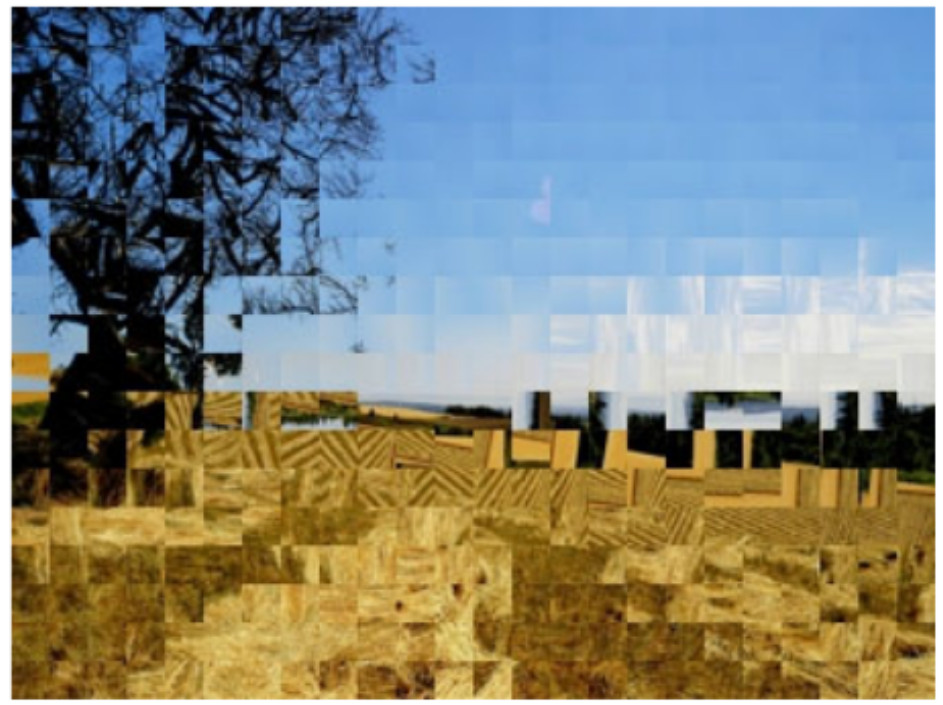
\includegraphics[width=\linewidth]{20-prologue/puzzlerotation.jpg}
    \caption[A rotation prediction task]{Example of input in the case the position is known but the rotation is unknown. © A.C. Gallagher \citep{gallagher2012jigsaw}.}
    \label{fig:pstask:rotation}
\end{marginfigure}

    \item[Fragments quantity:] text
    \item[Binding puzzle sizes:] text
\end{description}

% -------------------------------------------------------

\subsection{Bullet list}

\begin{itemize}
    \item archaeology;
    \item cryptography;
    \item forensic medicine;
    \item genome biology;
    \item medicine.
\end{itemize}
